In der hochaufgelösten Resonanz-Ionisations-Spektroskopie ist es
sehr wichtig, über längere Messzeiten möglichst konstante Rahmenbedingungen für die Messung zu
schaffen. Auch die Reproduzierbarkeit von Messungen ist nur gewährleistet, wenn
die Experimentparameter konstant bleiben. Ein wesentlicher, wenn nicht der
wichtigste, Parametersatz des Experiments sind die Lasereigenschaften. Für
eine stabile Laserfrequenz ist die Stabilität des Resonators ausschlaggebend.
Vibrationen, Luftdichte- bzw. Verstärungsmediumsdichtefluktuationen und
Brechungsindexänderungen, hervorgerufen durch Temperaturschwankungen, sind für
Instabilitäten verantwortlich. Schon bei Schwankungen oder Drifts von wenigen
MHz kann es bei sehr schmalbandigen Atomaren Übergängen zu erheblichen
Fluktuationen in der Ionisatonsrate kommen. Daher ist eine aktive
Frequenzstabilisierung der Diodenlaser unerlässlich.\par
In diesem Kapitel sollen zunächst der Vollständigkeit halber bewährte
Frequenzstabilisierungstechniken wie
\textit{Hänsch-Couillaud} (Kap.
\ref{sec:haensch-couillaud}) und \textit{Pound-Drever-Hall} (Kap.
\ref{sec:pound-drever-hall}) kurz vorgestellt
(\cite{noertershaeuser:physik_des_lasers}) und anschließend auf das
in diesem Projekt verwendete \textit{Fringe-Offset-Locking} (Kap.
\ref{sec:fringe-offset-locking}) näher eingegangen werden. Darüber hinaus
besteht auch die Anforderung, zwischen den Anregungsfrequenzen verschiedener
Isotope möglichst schnell wechseln zu können. Dies ist allein mit der
Fringe-Offset-Locking nur bedingt gegeben. Deshalb wurde diese Technik mit einer
kommerziellen Stabilisierunugstechnik kombiniert, auf die und deren Kombination
mit der Fringe-Offset-Technik am Ende dieses Kapitals eingegangen wird.\par
Um einen Laser auf einer Frequenz festzuhalten, benötigt
man eine Referenz. Diese kann ein passiver, stabiler Resonator, ein atomarer
bzw. molekularer Übergang oder ein absolut stabiler Laser wie z.B. ein
Helium-Neon-Laser (He:Ne-Laser) sein.
Aus der Abweichung der Frequenz des zu stabilisierenden Lasers $\nu_{ist}$ zur
Sollfrequenz $\nu_{soll}$ muss ein Fehlersignal
\begin{equation}\label{eq:servoschleife_fehlersignal}
	S\approx C\cdot(\nu_{ist}-\nu_{soll})=C\cdot\delta\nu
\end{equation}
erzeugt werden, das hier exemplarisch linear zur Frequenzdifferenz $\delta\nu$
ist. Dieses Fehlersignal dient als Eingangssignal für eine Regelschleife, die
die Frequenz des Lasers auf die Sollfrequenz regelt. Auf Details dieser
Regelschleife soll später genauer eingegangen werden (siehe
\ref{sec:regeltechnik}). Die Generierung des Fehlersignals kann auf verschiedene Arten geschehen, wie im Folgenden zu sehen
ist.

\section{Hänsch-Couillaud}\label{sec:haensch-couillaud}
\begin{figure}[h]
 	\centering
 	\fbox{\parbox{\dimexpr \linewidth - 2\fboxrule - 2\fboxsep}{
 	\centering
	    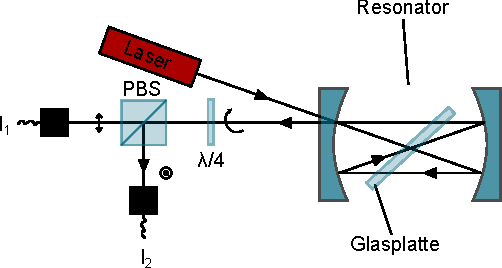
\includegraphics[width=\textwidth-4cm]{gfx/haensch-couillaud_aufbau}
	}}
	\caption[Hänsch-Couillaud - Aufbau]{Aufbau
	einer Frequenzstabilisierung nach Hänsch
	und Couillaud. Erkläung im Text.}\label{fig:haensch-couillaud_aufbau}
\end{figure}
Die Frequenzstabilisierung nach Hänsch und Couillaud (HC)
basiert auf der \textit{Polarisationsspektroskopie}. Mit Hilfe eines
optischen Elemtents in einem festen Resonators als Referenz können verschiedene
Polarisationen des Laserlichts verschiedene Verluste erfahren. Dies lässt sich
mit einem doppelbrechenden Kristall oder einer Glasscheibe im Brewsterwinkel
realisieren. Man kann das elektrische Feld des linear polarisierten einfallenden
Lichts $E_0$ in Komponenten senkrecht und parallel zur Polarisationsrichtung mit
minimalen Verlusten zerlegen:
\begin{equation}\label{eq:haensch-couillaud_01}
	\begin{split}
		E_{\perp}^{(0)} & = E_0\cdot\cos{(\Theta)}\\
		E_{\parallel}^{(0)} & = E_0\cdot\sin{(\Theta)}\,.
	\end{split}
\end{equation}
Dabei ist $\Theta$ der Winkel zwischen einfallender Polarisation und
Polarisation mit maximalen bzw. minimalen Verlusten. $E_{\perp}^{(0)}$ wird also
im Wesentlichen vom Einkoppelspiegel reflektiert. $E_{\parallel}^{(0)}$
wird hingegen in den Resonator eingekoppelt und erfärt bei Nicht-Resonanz im
Resonator eine Phasenverschiebung $\delta$ zu $E_{\perp}^{(0)}$. Im Resonanzfall
ist diese Phasenverschiebung null. Durch Kenntnis der Phasenverschiebung kann
also eine Aussage über die Verstimmung zur Resonanz getroffen werden. Die
Komponenten des refelktierten Lichts
\begin{equation}\label{eq:haensch-couillaud_02}
	\begin{split}
		E_{\perp}^{(r)} & = E_{\perp}^{(0)}\cdot r_1\\
		E_{\parallel}^{(r)} & = E_{\parallel}^{(0)}\cdot\left(r_1-\frac{t_1^2r\mathrm{e}^{-\mathrm{i}\delta}}{r_1\left(1-r\mathrm{e}^{-\mathrm{i}\delta}\right)}\right)
	\end{split}
\end{equation}
ergeben zusammen elliptisch polarisiertes Licht und somit eine Überlagerung von
$\sigma^+$- und $\sigma^-$-Licht mit unterschiedlichen Amplituden. Dabei sind
$r_1$ und $t_1$ Reflexions- und Transmissionskoeffizienten des
Einkoppelspiegels. $r$ beschreibt die Verluste durch die Umläufe im Resonator.
Bei Phasenverschiebung überwiegt einmal der $\sigma^+$-Anteil und einmal der $\sigma^-$-Anteil. Bei Resonanz sind beide Anteile gleich und es entsteht wieder linear polarisiertes Licht. Eine $\nicefrac{\lambda}{4}$-Platte erzeugt aus
beiden zirkularen Anteilen ($\sigma^+$ und $\sigma^-$) lineare Anteile, welche
durch einen Polarisationsstrahlteiler getrennt und letzendlich durch Photodioden
detektiert werden können. Abbildung \ref{fig:haensch-couillaud_aufbau} zeigt den
optischen Aufbau. Die Differenz der zu den Feldstärken der elektrischen Komponente
des Lichts proportionalen Ströme der Photodioden
\begin{equation}\label{eq:haensch-couillaud_fehlersignal}
	(I_1-I_2)\propto\abs{E^{(0)}}^2\cos{(\Theta)}\sin{(\Theta)}\frac{t_1^2r^2\sin{(\delta)}}{(1-r^2)+4r^2\sin^2{\left(\frac{\delta}{2}\right)}}
\end{equation}
lieftert das in Abb. \ref{fig:haensch-couillaud_fehlersignal} gezeichnete
Fehlersignal mit Nulldurchgang bei den Resonanzen $\delta=2\pi n$. Die
Regelschleife muss also auf diesen Nulldurchgang regeln.
\begin{figure}[h]
	\centering
	\footnotesize
	% GNUPLOT: LaTeX picture with Postscript
\begingroup
  \makeatletter
  \providecommand\color[2][]{%
    \GenericError{(gnuplot) \space\space\space\@spaces}{%
      Package color not loaded in conjunction with
      terminal option `colourtext'%
    }{See the gnuplot documentation for explanation.%
    }{Either use 'blacktext' in gnuplot or load the package
      color.sty in LaTeX.}%
    \renewcommand\color[2][]{}%
  }%
  \providecommand\includegraphics[2][]{%
    \GenericError{(gnuplot) \space\space\space\@spaces}{%
      Package graphicx or graphics not loaded%
    }{See the gnuplot documentation for explanation.%
    }{The gnuplot epslatex terminal needs graphicx.sty or graphics.sty.}%
    \renewcommand\includegraphics[2][]{}%
  }%
  \providecommand\rotatebox[2]{#2}%
  \@ifundefined{ifGPcolor}{%
    \newif\ifGPcolor
    \GPcolortrue
  }{}%
  \@ifundefined{ifGPblacktext}{%
    \newif\ifGPblacktext
    \GPblacktexttrue
  }{}%
  % define a \g@addto@macro without @ in the name:
  \let\gplgaddtomacro\g@addto@macro
  % define empty templates for all commands taking text:
  \gdef\gplbacktext{}%
  \gdef\gplfronttext{}%
  \makeatother
  \ifGPblacktext
    % no textcolor at all
    \def\colorrgb#1{}%
    \def\colorgray#1{}%
  \else
    % gray or color?
    \ifGPcolor
      \def\colorrgb#1{\color[rgb]{#1}}%
      \def\colorgray#1{\color[gray]{#1}}%
      \expandafter\def\csname LTw\endcsname{\color{white}}%
      \expandafter\def\csname LTb\endcsname{\color{black}}%
      \expandafter\def\csname LTa\endcsname{\color{black}}%
      \expandafter\def\csname LT0\endcsname{\color[rgb]{1,0,0}}%
      \expandafter\def\csname LT1\endcsname{\color[rgb]{0,1,0}}%
      \expandafter\def\csname LT2\endcsname{\color[rgb]{0,0,1}}%
      \expandafter\def\csname LT3\endcsname{\color[rgb]{1,0,1}}%
      \expandafter\def\csname LT4\endcsname{\color[rgb]{0,1,1}}%
      \expandafter\def\csname LT5\endcsname{\color[rgb]{1,1,0}}%
      \expandafter\def\csname LT6\endcsname{\color[rgb]{0,0,0}}%
      \expandafter\def\csname LT7\endcsname{\color[rgb]{1,0.3,0}}%
      \expandafter\def\csname LT8\endcsname{\color[rgb]{0.5,0.5,0.5}}%
    \else
      % gray
      \def\colorrgb#1{\color{black}}%
      \def\colorgray#1{\color[gray]{#1}}%
      \expandafter\def\csname LTw\endcsname{\color{white}}%
      \expandafter\def\csname LTb\endcsname{\color{black}}%
      \expandafter\def\csname LTa\endcsname{\color{black}}%
      \expandafter\def\csname LT0\endcsname{\color{black}}%
      \expandafter\def\csname LT1\endcsname{\color{black}}%
      \expandafter\def\csname LT2\endcsname{\color{black}}%
      \expandafter\def\csname LT3\endcsname{\color{black}}%
      \expandafter\def\csname LT4\endcsname{\color{black}}%
      \expandafter\def\csname LT5\endcsname{\color{black}}%
      \expandafter\def\csname LT6\endcsname{\color{black}}%
      \expandafter\def\csname LT7\endcsname{\color{black}}%
      \expandafter\def\csname LT8\endcsname{\color{black}}%
    \fi
  \fi
  \setlength{\unitlength}{0.0500bp}%
  \begin{picture}(7200.00,5040.00)%
    \gplgaddtomacro\gplbacktext{%
      \csname LTb\endcsname%
      \put(860,1120){\makebox(0,0)[r]{\strut{}-1}}%
      \put(860,1920){\makebox(0,0)[r]{\strut{}-0.5}}%
      \put(860,2719){\makebox(0,0)[r]{\strut{} 0}}%
      \put(860,3519){\makebox(0,0)[r]{\strut{} 0.5}}%
      \put(860,4319){\makebox(0,0)[r]{\strut{} 1}}%
      \put(980,440){\makebox(0,0){\strut{}-3}}%
      \put(1957,440){\makebox(0,0){\strut{}-2}}%
      \put(2933,440){\makebox(0,0){\strut{}-1}}%
      \put(3910,440){\makebox(0,0){\strut{} 0}}%
      \put(4886,440){\makebox(0,0){\strut{} 1}}%
      \put(5863,440){\makebox(0,0){\strut{} 2}}%
      \put(6839,440){\makebox(0,0){\strut{} 3}}%
      \put(160,2719){\rotatebox{-270}{\makebox(0,0){\strut{}Amplitude}}}%
      \put(3909,140){\makebox(0,0){\strut{}Phasenverschiebung relativ zur Resonanz $\nicefrac{\delta}{\pi}$}}%
    }%
    \gplgaddtomacro\gplfronttext{%
    }%
    \gplbacktext
    \put(0,0){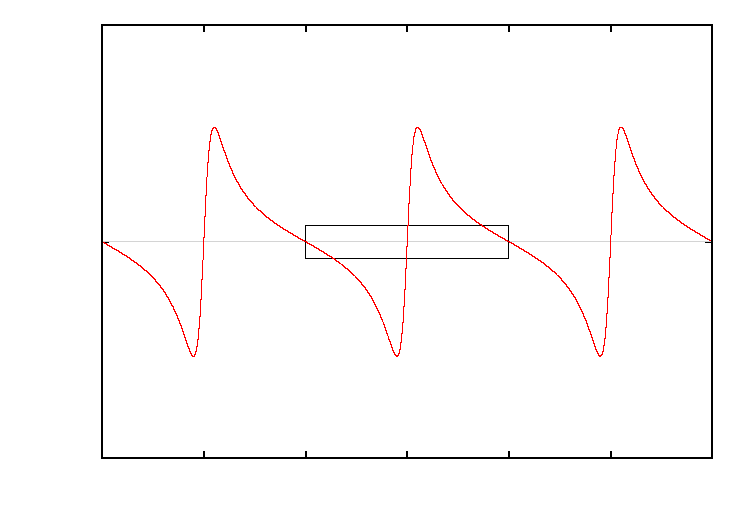
\includegraphics{haensch-couillaud_fehlersignal}}%
    \gplfronttext
  \end{picture}%
\endgroup

	\caption[Hänsch-Couillaud
	Fehlersignal]{Fehlersignal der
	Hänsch-Couillaud-Stabilisierung
	gemäß Gl.
	\eqref{eq:haensch-couillaud_fehlersignal}.
	Der markierte Bereich ist der
	Fangbereich der Regelung.}\label{fig:haensch-couillaud_fehlersignal}
\end{figure}

\section{Pound-Drever-Hall}\label{sec:pound-drever-hall}
\begin{figure}[h]
 	\centering
 	\fbox{\parbox{\dimexpr \linewidth - 2\fboxrule - 2\fboxsep}{
 	\centering
	    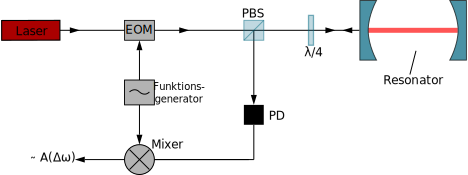
\includegraphics[width=\textwidth-0.5cm]{gfx/pound-drever-hall_aufbau}
	}}
	\caption[Pound-Drever-Hall - Aufbau]{Aufbau
	einer Frequenzstabilisierung nach Pound, Drever und Hall. Erkläung im
	Text.}\label{fig:pound-drever-hall_aufbau}
\end{figure}
Ein Aufbau des Verfahrens nach Pound, Drever und Hall (PDH) ist in Abb.
\ref{fig:pound-drever-hall_aufbau} dargestellt.
Das Laserlicht mit der Frequenz $\omega_L$ wird mittels eines \textit{elektrooptischen Modulators}, kurz EOM, in der Phase gemäß
\begin{equation}\label{eq:pound-drever-hall_01}
	E=\E_0\cos{\left(\omega_Lt+\delta\cos{(\omega_mt)}\right)}
\end{equation}
mit einem kleinen Modulationsindex $\delta\ll1$ moduliert. Dabei treten in
erster Ordnung gegenphasige Seitenbänder mit der Frequenz $\omega_L\pm\omega_m$
auf. Als Referenz dient wieder wie oben ein Resonator, in den bei Resonanz ein
Teil des Trägerlichts eingekoppelt wird. Die Seitenbänder und der restliche Teil
des Trägers werden refelektiert. Da bei Resonanz das Licht im Resonator einen
Phasensprung von $\pi$ erfährt, ergibt sich für die Nettoleistung des
refelktierten Trägerlichts eine Abschwächung durch destruktive Interferenz.
Da die beiden Seitenbänder gegenphasig schwingen, haben die Schwebungen dieser
Seitenbänder mit dem Träger unterschiedliche Vorzeichen. Im Resonanzfall heben
sich also die Schwebungssignale aufgrund gleicher Amplitude gegenseitig auf, was
zu vollständiger destruktiver Interferenz führt. Bei geringer Verstimmung des
Lasersfrequenz zur Resonanzfrequenz des Resonators, ist die Phasenverschiebung
im Resonator nicht mehr $\pi$, was zu unterschiedlichen Amplituden der
Schwebungssignale führt. Das resultierende Signal ist also von null
verschieden.\par
Die Trennung des einfallenden Lichts vom zu analysierenden Licht kann mit einer
$\nicefrac{\lambda}{4}$-Platte und einem Polarisationsstrahlteiler realisiert
werden. Für den Photodiodenstrom erhält man in Abhängigkeit von der Verstimmtung
des Trägerlichts zur Resonanz
\begin{equation}\label{eq:pound-drever-hall_fehlersignal}
	I(\Delta\omega,\omega_m)\propto
	J_0(\delta)J_1(\delta)\left[A(\Delta\omega)\cos{(\omega_mt)}+D(\Delta\omega)\sin{(\omega_mt)}\right]\,,
\end{equation}
wobei $J_{0,1}$ nullte und erste Ordnung von Besselfunktionen sind. Mischt man
das Signal mit dem der Modulation, erhält man als Ausgangssignal den zur
Modulation gleichphasigen Anteil von
Gl. \eqref{eq:pound-drever-hall_fehlersignal}, der proportional zu
$A(\Delta\omega)$ ist.
Abbildung \ref{fig:pound-drever-hall_fehlersignal} zeigt die Abhängigkeit dieses
Fehlsignals zur Verstimmung $\Delta\omega$. Um den Laser auf Resonanz zu halten,
muss auf den Nulldurchgang geregelt werden.
\begin{figure}[h]
	\centering
	\footnotesize
	% GNUPLOT: LaTeX picture with Postscript
\begingroup
  \makeatletter
  \providecommand\color[2][]{%
    \GenericError{(gnuplot) \space\space\space\@spaces}{%
      Package color not loaded in conjunction with
      terminal option `colourtext'%
    }{See the gnuplot documentation for explanation.%
    }{Either use 'blacktext' in gnuplot or load the package
      color.sty in LaTeX.}%
    \renewcommand\color[2][]{}%
  }%
  \providecommand\includegraphics[2][]{%
    \GenericError{(gnuplot) \space\space\space\@spaces}{%
      Package graphicx or graphics not loaded%
    }{See the gnuplot documentation for explanation.%
    }{The gnuplot epslatex terminal needs graphicx.sty or graphics.sty.}%
    \renewcommand\includegraphics[2][]{}%
  }%
  \providecommand\rotatebox[2]{#2}%
  \@ifundefined{ifGPcolor}{%
    \newif\ifGPcolor
    \GPcolortrue
  }{}%
  \@ifundefined{ifGPblacktext}{%
    \newif\ifGPblacktext
    \GPblacktexttrue
  }{}%
  % define a \g@addto@macro without @ in the name:
  \let\gplgaddtomacro\g@addto@macro
  % define empty templates for all commands taking text:
  \gdef\gplbacktext{}%
  \gdef\gplfronttext{}%
  \makeatother
  \ifGPblacktext
    % no textcolor at all
    \def\colorrgb#1{}%
    \def\colorgray#1{}%
  \else
    % gray or color?
    \ifGPcolor
      \def\colorrgb#1{\color[rgb]{#1}}%
      \def\colorgray#1{\color[gray]{#1}}%
      \expandafter\def\csname LTw\endcsname{\color{white}}%
      \expandafter\def\csname LTb\endcsname{\color{black}}%
      \expandafter\def\csname LTa\endcsname{\color{black}}%
      \expandafter\def\csname LT0\endcsname{\color[rgb]{1,0,0}}%
      \expandafter\def\csname LT1\endcsname{\color[rgb]{0,1,0}}%
      \expandafter\def\csname LT2\endcsname{\color[rgb]{0,0,1}}%
      \expandafter\def\csname LT3\endcsname{\color[rgb]{1,0,1}}%
      \expandafter\def\csname LT4\endcsname{\color[rgb]{0,1,1}}%
      \expandafter\def\csname LT5\endcsname{\color[rgb]{1,1,0}}%
      \expandafter\def\csname LT6\endcsname{\color[rgb]{0,0,0}}%
      \expandafter\def\csname LT7\endcsname{\color[rgb]{1,0.3,0}}%
      \expandafter\def\csname LT8\endcsname{\color[rgb]{0.5,0.5,0.5}}%
    \else
      % gray
      \def\colorrgb#1{\color{black}}%
      \def\colorgray#1{\color[gray]{#1}}%
      \expandafter\def\csname LTw\endcsname{\color{white}}%
      \expandafter\def\csname LTb\endcsname{\color{black}}%
      \expandafter\def\csname LTa\endcsname{\color{black}}%
      \expandafter\def\csname LT0\endcsname{\color{black}}%
      \expandafter\def\csname LT1\endcsname{\color{black}}%
      \expandafter\def\csname LT2\endcsname{\color{black}}%
      \expandafter\def\csname LT3\endcsname{\color{black}}%
      \expandafter\def\csname LT4\endcsname{\color{black}}%
      \expandafter\def\csname LT5\endcsname{\color{black}}%
      \expandafter\def\csname LT6\endcsname{\color{black}}%
      \expandafter\def\csname LT7\endcsname{\color{black}}%
      \expandafter\def\csname LT8\endcsname{\color{black}}%
    \fi
  \fi
  \setlength{\unitlength}{0.0500bp}%
  \begin{picture}(7200.00,5040.00)%
    \gplgaddtomacro\gplbacktext{%
      \csname LTb\endcsname%
      \put(860,1056){\makebox(0,0)[r]{\strut{}-0.4}}%
      \put(860,1888){\makebox(0,0)[r]{\strut{}-0.2}}%
      \put(860,2719){\makebox(0,0)[r]{\strut{} 0}}%
      \put(860,3551){\makebox(0,0)[r]{\strut{} 0.2}}%
      \put(860,4383){\makebox(0,0)[r]{\strut{} 0.4}}%
      \put(980,440){\makebox(0,0){\strut{}-10}}%
      \put(2445,440){\makebox(0,0){\strut{}-5}}%
      \put(3909,440){\makebox(0,0){\strut{} 0}}%
      \put(5374,440){\makebox(0,0){\strut{} 5}}%
      \put(6839,440){\makebox(0,0){\strut{} 10}}%
      \put(160,2719){\rotatebox{-270}{\makebox(0,0){\strut{}$A(\Delta\omega)$}}}%
      \put(3909,140){\makebox(0,0){\strut{}Verstimmung zur Resonanz $\Delta\omega$}}%
    }%
    \gplgaddtomacro\gplfronttext{%
    }%
    \gplbacktext
    \put(0,0){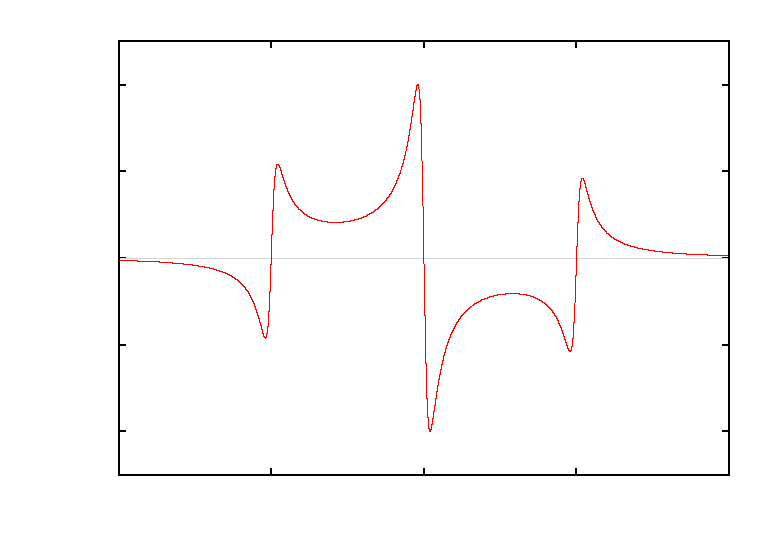
\includegraphics{pound-drever-hall_fehlersignal}}%
    \gplfronttext
  \end{picture}%
\endgroup

	\caption[Hänsch-Couillaud
	Fehlersignal]{Fehlersignal der
	Pound-Drever-Hall-Stabilisierung
	gemäß Gl.
	\eqref{eq:pound-drever-hall_fehlersignal}. Die Modulation 
	$\pm\omega_m$ liegt bei $\pm5$.}\label{fig:pound-drever-hall_fehlersignal}
\end{figure}

\section{Fringe-Offset-Locking}\label{sec:fringe-offset-locking}
Die oben erklärten Techniken sind darauf ausgelegt einen einzigen Laser zu
stabilisieren. Ein Frequenzscan ist bei der PDH-Methode nur sehr eingeschränkt
möglich. Der Referenz-Resonator müsste sehr langsam verstimmt werden, damit die
Regelung nach kommt. Größere Frequenzsprünge sind auch bei der HC-Methode auch
nur bedingt möglich. Hier wird allerdings eine Stabilisierung benötigt, die drei
Laser unabhängig voneinander kontrollieren kann. Schnelles Verfahren auf
gewünschte Relativfrequenzen sind auch gefordert. Aus Kosten- und
Aufwandsgründen ist es auch von Vorteil, wenn für alle drei Laser dieselbe
Referenz verwendet werden können, ohne, dass sie voneinander abhängig sind. Eine
hervorragende Methode dafür ist das Fringe-Offset-Locking. Diese Methode soll im
Folgenden genauer betrachtet werden.

\subsection{Fabry-Perot-Interferometer}
Eine entscheidende Rolle spielt hier ein sog.
\textit{Fabry-Perot-Interferometer}, kurz FPI, das sowohl
als feste Referenenz als auch als Frequenzspektrum-Analysator dienen kann.
Beide Varianten sollen in diesem Kapitel vorgestellt werden. Die Ausführungen
stützen sich auf die Arbeiten \cite{wiche:1997:diplomarbeit} und
\cite{kuschnick:2000:diplomarbeit}.

\subsubsection{Festes FPI}\label{subsubsec:festes_FPI}
Ein FPI ist ein Resonator bestehend aus zwei planparallelen Spiegeln mit den
Reflektivitäten $R_1$ und $R_2$ und dem Abstand $L$ wie in Abb.
\ref{fig:FPI_planparallel} schematisch dargestellt.
\begin{figure}[h]
 	\centering
 	\fbox{\parbox{\dimexpr \linewidth - 2\fboxrule - 2\fboxsep}{
 	\centering
	    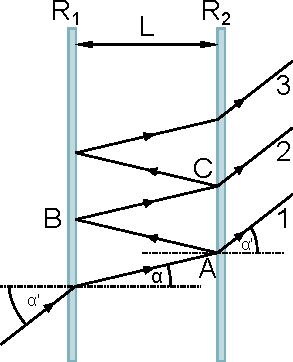
\includegraphics[width=7cm]{gfx/FPI_planparallel}
	}}
	\caption[FPI - planparallel]{Strahlengang in einem
	planprarallelen Fabry-Perot-Interferometer.}\label{fig:FPI_planparallel}
\end{figure}
Licht, das unter dem Winkel
$\alpha'$ von links eingestrahlt wird, wird nach dem Gesetz von Snellius
\begin{equation}\label{eq:snellius}
	\frac{n_r}{n_{ext}}=\frac{\sin{(\alpha')}}{\sin{(\alpha)}}
\end{equation}
auf den Winkel $\alpha$ gebrochen, wenn $n_r$ bzw. $n_{ext}$ der Brechungsindex
des Resonators bzw. der Raumluft ist. Der Resonator in diesem Experiment ist
zwecks Unterdrückung der Schwankungen des Brechungsindexes evakuiert, wodurch
$n_r\approx1$ gilt. Aus Vollständigkeitsgründen soll $n_r$ aber weiterhin
Parameter bleiben. Für die Amplitude des elektrischen Feldes $E_1$ des direkt
transmittierten Lichts ergibt sich
\begin{equation}\label{eq:FPI_E1}
	E_1=E_0t_1t_2\mathrm{e}^{\mathrm{i}\phi'}\,.
\end{equation}
Hierbei ist $E_0$ die Amplitude des elektrischen Feldes des Lichts, $t_1$ und
$t_2$ die Transmissionskoeffizienten bezüglich des elektrischen Feldes der
beiden Spiegel und $\phi'$ die Phasenänderung elektromagnetischen Welle nach
direkter Transmission des FPIs. Für die Amplitude des elektrischen Feldes des
transmittierten Lichts nach einem Umlauf gilt
\begin{equation}\label{eq:FPI_E2}
	\begin{split}
		E_2
		&=E_0t_1r_2r_1t_2\mathrm{e}^{\mathrm{i}\phi'}\mathrm{e}^{\mathrm{i}2\phi}\\
		&=E_1r_1r_2\mathrm{e}^{\mathrm{i}2\phi}\,.
	\end{split}
\end{equation}
$2\phi$ ist hier die Phasenverschiebung, die das Licht nach einem Umlauf im
Resonator (A$\rightarrow$B$\rightarrow$C) erhält. Allgemein gilt für den m-ten
transmittierten Strahl
\begin{equation}\label{eq:FPI_Em}
	E_m=E_1(r_1r_2)^m\mathrm{e}^{\mathrm{i}m2\phi}\,.
\end{equation}
Die Phasenverschiebung $2\phi=kL_{opt}$ ist abhängig von der optischen Weglänge
$L_{opt}=\overline{AB}+\overline{BC}=\frac{2n_rL}{\cos{(\alpha)}}$ und der Wellenzahl des
Lichts $k=2\pi\frac{\nu}{c}$. Somit ergibt sich also
\begin{equation}\label{eq:FPI_phase}
	\phi=\frac{2\pi n_r\nu L}{\cos{(\alpha)}c}\,.
\end{equation}
Das gesamte elektrische Feld des transmittierten Lichts ist eine Superposition
aller transmittierter Einzelfelder:
\begin{equation}\label{eq:FPI_Et}
	\begin{split}
		E_t
		&=E_1\cdot\sum\limits_{m=0}^\infty(r_1r_2)^m\mathrm{e}^{\mathrm{i}2m\phi}\\
		&=E_1\frac{1}{1-r_1r_2\mathrm{e}^{\mathrm{i}2\phi}}\,.
	\end{split}
\end{equation}
Für die gesamte transmittierte Leistung folgt also
\begin{equation}\label{eq:FPI_transmission}
	\begin{split}
		T=\frac{\abs{E_t}^2}{\abs{E_0}^2}
		&=\frac{t_1^2t_2^2}{1-2r_1r_2\cos{(2\phi)}+r_1^2r_2^2}\\
		&=\frac{(1-R_1)(1-R_2)}{\left(1-\sqrt{R_1R_2}\right)^2+4\sqrt{R_1R_2}\sin^2{\phi}}\\
		&\text{mit}\quad
		R_i=r_i^2
		\quad\text{und}\quad
		t_i^2=1-r_i^2=1-R_i\,.
	\end{split}
\end{equation}
Setzt man nun gleiche Reflektivitäten der beiden Spiegel $R_1=R_2=R$ vorraus und
substituiert $\kappa:=\frac{4R}{(1-R)^2}$ erhält man die sog.
\textit{Airy-Funktion}
\begin{equation}\label{eq:FPI_airy-funktion}
	T=\frac{1}{1+\kappa\sin^2{(\phi)}}\,.
\end{equation}
Wie leicht zu erkennen ist, ist die Transmissions-Funktion $\pi$-periodisch in
der Phase $\phi$ und gleichzeitig in der Frequenz des Lasers, da die Phase nach
Gl. \eqref{eq:FPI_phase} frequenzabhängig ist. Abbildung
\ref{fig:airy-funktion} zeigt die Airy-Funktion für verschiedene Finessen
$F$ bzw. Reflektivitäten der Spiegel.
\begin{figure}[h]
	\centering
	\footnotesize
	% GNUPLOT: LaTeX picture with Postscript
\begingroup
  \makeatletter
  \providecommand\color[2][]{%
    \GenericError{(gnuplot) \space\space\space\@spaces}{%
      Package color not loaded in conjunction with
      terminal option `colourtext'%
    }{See the gnuplot documentation for explanation.%
    }{Either use 'blacktext' in gnuplot or load the package
      color.sty in LaTeX.}%
    \renewcommand\color[2][]{}%
  }%
  \providecommand\includegraphics[2][]{%
    \GenericError{(gnuplot) \space\space\space\@spaces}{%
      Package graphicx or graphics not loaded%
    }{See the gnuplot documentation for explanation.%
    }{The gnuplot epslatex terminal needs graphicx.sty or graphics.sty.}%
    \renewcommand\includegraphics[2][]{}%
  }%
  \providecommand\rotatebox[2]{#2}%
  \@ifundefined{ifGPcolor}{%
    \newif\ifGPcolor
    \GPcolortrue
  }{}%
  \@ifundefined{ifGPblacktext}{%
    \newif\ifGPblacktext
    \GPblacktexttrue
  }{}%
  % define a \g@addto@macro without @ in the name:
  \let\gplgaddtomacro\g@addto@macro
  % define empty templates for all commands taking text:
  \gdef\gplbacktext{}%
  \gdef\gplfronttext{}%
  \makeatother
  \ifGPblacktext
    % no textcolor at all
    \def\colorrgb#1{}%
    \def\colorgray#1{}%
  \else
    % gray or color?
    \ifGPcolor
      \def\colorrgb#1{\color[rgb]{#1}}%
      \def\colorgray#1{\color[gray]{#1}}%
      \expandafter\def\csname LTw\endcsname{\color{white}}%
      \expandafter\def\csname LTb\endcsname{\color{black}}%
      \expandafter\def\csname LTa\endcsname{\color{black}}%
      \expandafter\def\csname LT0\endcsname{\color[rgb]{1,0,0}}%
      \expandafter\def\csname LT1\endcsname{\color[rgb]{0,1,0}}%
      \expandafter\def\csname LT2\endcsname{\color[rgb]{0,0,1}}%
      \expandafter\def\csname LT3\endcsname{\color[rgb]{1,0,1}}%
      \expandafter\def\csname LT4\endcsname{\color[rgb]{0,1,1}}%
      \expandafter\def\csname LT5\endcsname{\color[rgb]{1,1,0}}%
      \expandafter\def\csname LT6\endcsname{\color[rgb]{0,0,0}}%
      \expandafter\def\csname LT7\endcsname{\color[rgb]{1,0.3,0}}%
      \expandafter\def\csname LT8\endcsname{\color[rgb]{0.5,0.5,0.5}}%
    \else
      % gray
      \def\colorrgb#1{\color{black}}%
      \def\colorgray#1{\color[gray]{#1}}%
      \expandafter\def\csname LTw\endcsname{\color{white}}%
      \expandafter\def\csname LTb\endcsname{\color{black}}%
      \expandafter\def\csname LTa\endcsname{\color{black}}%
      \expandafter\def\csname LT0\endcsname{\color{black}}%
      \expandafter\def\csname LT1\endcsname{\color{black}}%
      \expandafter\def\csname LT2\endcsname{\color{black}}%
      \expandafter\def\csname LT3\endcsname{\color{black}}%
      \expandafter\def\csname LT4\endcsname{\color{black}}%
      \expandafter\def\csname LT5\endcsname{\color{black}}%
      \expandafter\def\csname LT6\endcsname{\color{black}}%
      \expandafter\def\csname LT7\endcsname{\color{black}}%
      \expandafter\def\csname LT8\endcsname{\color{black}}%
    \fi
  \fi
  \setlength{\unitlength}{0.0500bp}%
  \begin{picture}(7200.00,5040.00)%
    \gplgaddtomacro\gplbacktext{%
      \csname LTb\endcsname%
      \put(540,830){\makebox(0,0)[r]{\strut{}0}}%
      \put(540,1780){\makebox(0,0)[r]{\strut{}0.5}}%
      \put(540,2729){\makebox(0,0)[r]{\strut{}1}}%
      \put(1023,440){\makebox(0,0){\strut{} 0}}%
      \put(1932,440){\makebox(0,0){\strut{} 0.5}}%
      \put(2841,440){\makebox(0,0){\strut{} 1}}%
      \put(3749,440){\makebox(0,0){\strut{} 1.5}}%
      \put(4658,440){\makebox(0,0){\strut{} 2}}%
      \put(5567,440){\makebox(0,0){\strut{} 2.5}}%
      \put(6476,440){\makebox(0,0){\strut{} 3}}%
      \put(1023,4639){\makebox(0,0){\strut{}0}}%
      \put(2841,4639){\makebox(0,0){\strut{}300}}%
      \put(4658,4639){\makebox(0,0){\strut{}600}}%
      \put(6476,4639){\makebox(0,0){\strut{}900}}%
      \put(200,1739){\rotatebox{-270}{\makebox(0,0){\strut{}Transmission}}}%
      \put(3749,140){\makebox(0,0){\strut{}Phase $\nicefrac{\phi}{\pi}$}}%
      \put(3749,4938){\makebox(0,0){\strut{}Frequenz $\nu$ [MHz]}}%
      \put(1750,2957){\makebox(0,0)[l]{\strut{}FSR}}%
    }%
    \gplgaddtomacro\gplfronttext{%
      \csname LTb\endcsname%
      \put(1620,4226){\makebox(0,0)[r]{\strut{}$F=2$}}%
      \csname LTb\endcsname%
      \put(1620,3926){\makebox(0,0)[r]{\strut{}$F=10$}}%
      \csname LTb\endcsname%
      \put(1620,3626){\makebox(0,0)[r]{\strut{}$F=100$}}%
    }%
    \gplgaddtomacro\gplbacktext{%
      \csname LTb\endcsname%
      \put(3756,3368){\makebox(0,0)[r]{\strut{} 0}}%
      \put(3756,3677){\makebox(0,0)[r]{\strut{} 50}}%
      \put(3756,3986){\makebox(0,0)[r]{\strut{} 100}}%
      \put(3756,4295){\makebox(0,0)[r]{\strut{} 150}}%
      \put(3876,2921){\makebox(0,0){\strut{} 0}}%
      \put(4440,2921){\makebox(0,0){\strut{} 0.2}}%
      \put(5004,2921){\makebox(0,0){\strut{} 0.4}}%
      \put(5567,2921){\makebox(0,0){\strut{} 0.6}}%
      \put(6131,2921){\makebox(0,0){\strut{} 0.8}}%
      \put(6695,2921){\makebox(0,0){\strut{} 1}}%
      \put(3356,3708){\rotatebox{-270}{\makebox(0,0){\strut{}Finesse}}}%
      \put(5285,3280){\makebox(0,0){\strut{}Reflektivit{"a}t}}%
    }%
    \gplgaddtomacro\gplfronttext{%
    }%
    \gplbacktext
    \put(0,0){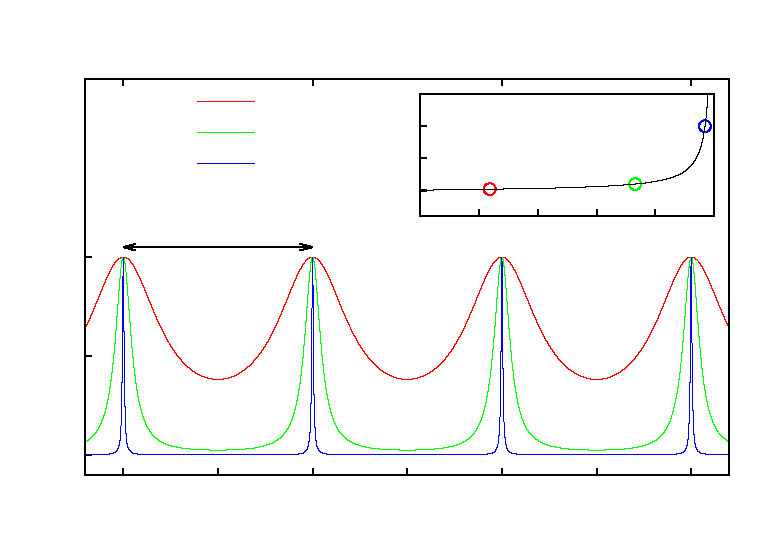
\includegraphics{airy-funktion}}%
    \gplfronttext
  \end{picture}%
\endgroup

	\caption[Airy-Funktion]{Airy-Funktion
	in Abhängigkeit von der Phase bzw.
	der Laserfrequenz. Eingezeichnet ist
	der freie Spektralbereich des
	Interferometers. Rechts oben ist die
	Finesse in Abhängigkeit zur
	Reflektivität der Spiegel dargestellt.}\label{fig:airy-funktion}
\end{figure}
Bei hoher Finesse sind scharfe
äquidistante Transmissionsmaxima zu erkennen. Mit der Annahme, dass das Licht
mit dem Winkel $\alpha'\ll1$ eingestrahlt wird, haben nach Gl.
\eqref{eq:FPI_phase} die Maxima $i$ einen Abstand von
\begin{equation}\label{eq:FPI_transmissionsmaxima}
	\Delta\nu=\abs{\nu_{i+1}-\nu_i}=\frac{c}{2\pi	n_rL}(\phi_{i+1}-\phi_i)=\frac{c}{2n_rL}\,.
\end{equation}
Dieser Frequenzabstand wird als \textit{freier Spektralbereich}, kurz FSR, des
FPIs bezeichnet und kann in Abhängigkeit von der optischen Weglänge $U$ für
einen Umlauf geschrieben werden:
\begin{equation}\label{eq:FPI_FSR_01}
	\text{FSR}=\frac{c}{U}
	\quad\text{mit}\quad
	U=2n_rL\,.
\end{equation}
In Abb. \ref{fig:airy-funktion} ist der FSR emeplarisch mit $300\,$MHz
angegeben. Damit das FPI unempfindlich auf kleine Variationen des Einfallswinkels $\alpha'$
ist, wird hier im Gegensatz zu einem planparallelen ein \textit{kofokales} FPI
verwendet wie es in Abb. \ref{fig:FPI_kofokal} dargestellt ist.
\begin{figure}[h]
 	\centering
 	\fbox{\parbox{\dimexpr \linewidth - 2\fboxrule - 2\fboxsep}{
 	\centering
	    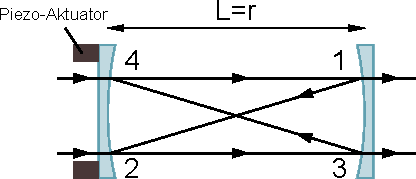
\includegraphics[width=\textwidth-4cm]{gfx/FPI_kofokal}
	}}
	\caption[FPI - planparallel]{Strahlengang in einem
	kofokalen Fabry-Perot-Interferometer. Die
	Krümmungsradien der Spiegel entsprechen dem
	Spiegelabstand. Ein ringförmiger Piezo-Aktuator dient zur
	Verstimmbarkeit des Spiegelabstands (vgl. Kap.
	\ref{subsubsec:scanning_FPI}).}\label{fig:FPI_kofokal}
\end{figure}
Der Abstand $L$ ist so gewählt, dass er den Spiegelradien entspricht und sich
ein gemeinsamer Fokus in der Mitte bildet. Da das Licht
in diesem Fall zwei Umläufe ($1\rightarrow2\rightarrow3\rightarrow4$)
benötigt, damit die transmittierten Felder interferieren können,
verdoppelt sich die optische Weglänge auf $U=4n_rL$, was zu einem FSR von
\begin{equation}\label{eq:FPI_FSR_02}
	\text{FSR}=\frac{c}{4n_rL}
\end{equation}
führt. Die eben schon erwähnte Finesse ist ein Maß für die Peakbreite der
Transmissionsfunktion \eqref{eq:FPI_airy-funktion} und wichtet den FSR mit der
inversen Halbwertsbreite der Peaks:
\begin{equation}\label{eq:FPI_finesse}
	F=\frac{\text{FSR}}{\Delta\nu_{\nicefrac{1}{2}}}\approx\frac{\pi\sqrt{R}}{1-R}
	\quad\text{für}\quad F\gg1\,.
\end{equation}
Ebenfalls ist die Finesse - wie in Abb. \ref{fig:airy-funktion} aufgetragen
- abhängig von der Reflektivität der Spiegel. Zu erkennen ist, dass hohe
Finessen erst bei Reflektivitäten nahe 1 erreicht werden.

\subsubsection{Scanning FPI}\label{subsubsec:scanning_FPI}
Als fester Resonator ist das FPI prinzipiell nichts anderes als die
Frequenz-Referenzen in Kap. \ref{sec:haensch-couillaud} und
\ref{sec:pound-drever-hall}. Es ist jedoch auch möglich anstatt durch
Verstimmung der Laserfrequenz durch Variation der Resonatorlänge
Transmissionsmaxima zu erhalten. Dies ist leicht aus der linearen Abhängigkeit
der Phase $\phi$ von der Resonatorlänge $L$ in Gl. \eqref{eq:FPI_phase}
ersichtlich. Die Längenveränderung ist mit einem ringförmigen Piezo-Aktuator
möglich, wie in \ref{fig:FPI_kofokal} eingezeichnet. Die Ausdehnung eines
Piezo-Aktuators ist nahezu linear in der Ladungsmenge, die auf ihn fließt, und
somit linear bei konstantem Stromfluss. Näherungsweise linear ist er allerdings
auch in der angelegten Spannung. Für ein kofokales FPI folgt für die Längenperioden $\Delta L$
benachbarter Transmissionsmaxima mit $\phi=\pi$
\begin{equation}\label{eq:FPI_laengenperiode}
	\Delta L=\frac{c}{4n_r\nu}=\frac{\lambda}{4n_r}\,.
\end{equation}
Die Längenperiode entspricht also einem Viertel der Wellenlänge, was sofort
einsichtig ist, da die Längenänderung somit für einen Umlauf genau $\lambda$ ist
und zur konstruktiven Interferenz führt. Mit dieser Information lässt sich nun
bei zeitlich linearer Längenvariation eine Eichung zwischen Zeit und Frequenz
machen
\begin{equation}\label{eq:FPI_zeit-eichung}
	\frac{\Delta T}{\Delta\nu}=\frac{\Delta T}{\Delta L}\cdot\frac{\Delta
	L}{\Delta\nu}=\frac{1}{v}\cdot\frac{-\lambda}{4n_r\text{FSR}}=\frac{-c}{4v\nu
	n_r\text{FSR}}=:\fracd{t}{\nu}\,,
\end{equation}
wobei $v$ die Geschwindigkeit ist, mit der sich der Piezo-Aktuator ausdehnt.
Das Minus folgt aus einer negativen Längenänderung des Interferometers
(Ausdehnung des Piezo-Aktuators).\par
Es ist also für das zeitliche Transmissionssignal unerheblich, ob man
Laserfrequenz oder Resonatorlänge variiert. Die Längenvariation birgt den großen
Vorteil, dass man das Verhalten mehrere Laser gleichzeitig überwachen kann,
sofern man eine weitere Referenz wie z.B. ein He:Ne-Laser verwendet.
Dabei müssen nur alle Laserstrahlen zusammengeführt das FPI durchlaufen und danach
wieder getrennt detektiert werden, wenn gleichzeitig die Länge des
Interferometers periodisch linear durchgefahren wird mit beispielsweise einer
Sägezahnspannung. Wie genau diese Laserkontrolle realisiert wird, soll im
folgenden Abschnitt näher erklärt werden.

\subsection{Relativfrequenzberechnung
und Laserkontrolle}\label{subsec:relativfrequenzberechnung_und_laserkontrolle}
In diesem Abschnitt werden das Funktionsprinzip des Fringe-Offset-Locking anhand
eines zu stabilisierenden Lasers und einem Referenzlaser beschrieben. Die
konkrete Realisierung soll in Kap. \ref{sec:elektronik_laserkontrolle}
detailliert vorgestellt werden.\par
\begin{figure}[h]
 	\centering
 	\fbox{\parbox{\dimexpr \linewidth - 2\fboxrule - 2\fboxsep}{
 	\centering
	    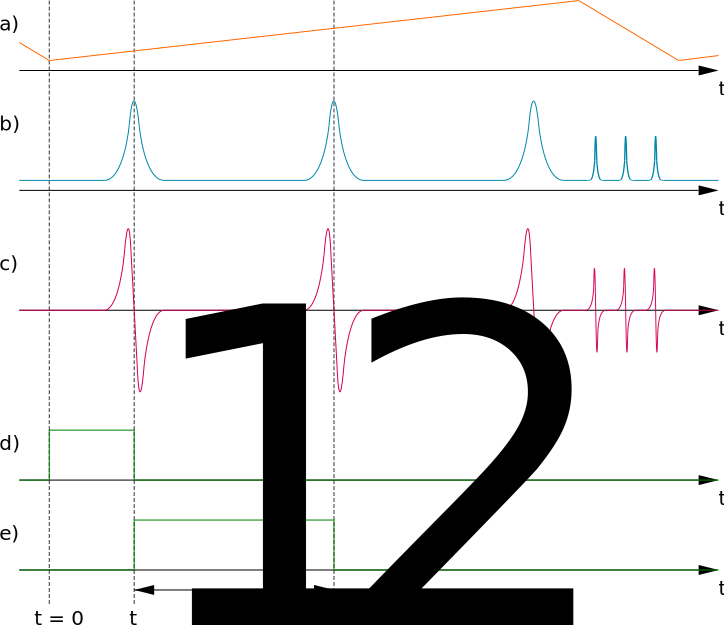
\includegraphics[width=\textwidth-4cm]{gfx/FPI_signal-zeitverlauf}
	}}
	\caption[Zeitlicher Verlauf
	FPI-Transmission]{Zeitlicher Verlauf der
	Transmissionssignale des FPIs. Erklärungen im Text.}\label{fig:FPI_signal-zeitverlauf}
\end{figure}
Um regelmäßig Informationen über die Laserfrequenz zu erhalten, wird der
Piezo-Aktuator des Interferometers periodisch mit einer asymmetrischen
Sägezahnspannung betrieben (Abb. \ref{fig:FPI_signal-zeitverlauf}(a)). Abbildung
\ref{fig:FPI_signal-zeitverlauf} zeigt den zeitlichen Verlauf der Signale eines
Lasers innerhalb eines Rampenzykluses. Sowohl für den zu stabilisierenden
Laser als auch für den Referenzlaser wird das zeitliche Transmisionssignal (im
Folgenden \textit{Fringepattern} genannt) mit einer Photodiode bei jeder
steigenden Spannungsflanke aufgenommen(Abb.
\ref{fig:FPI_signal-zeitverlauf}(b)). Der Beginn der steigenden Rampe ist der
Trigger für die Zeitskala. Die Positionen der Peaks (im Folgenden
\textit{Fringes} genannt) enthalten Information über die momentane
Laserfrequenz der zu stabilisierenden Laser. Allerdings können nur relative Frequenzänderungen zw.
verschiedenen Rampenzyklen und \textbf{keine} Absolutfrequenzen gemessen
werden. Um die Information zu verarbeiten, werden Ableitungen der Signale mit
steilen Nulldurchgängen generiert (Abb.
\ref{fig:FPI_signal-zeitverlauf}(c)).\par
Beim Start der Rampe werden die TTL-Signale für die \textit{Offsetfringes} der
beiden Laser auf HI gesetzt und damit jeweils ein Counter gestartet. Wird der
erste Fringe eines Lasers durch den Nulldurchgang seiner Ableitung detektiert,
so wird sein Offsetfringes-TTL-Signal auf LO gesetzt und der entsprechende
Counter gestoppt, wodurch man die Zeit $t_1$ erhält (Abb.
\ref{fig:FPI_signal-zeitverlauf}(d)). Zeitgleich wird das TTL-Signal des
\textit{Interfringes} auf HI gesetzt und ein zweiter Counter gestartet.
Folgt der zweite Fringe des entsprechenden Lasers, wird das
Interfringes-TTL-Signal auf LO gesetzt und auch der zweite Counter gestoppt, der
die Zeit $t_2-t_1$ liefert (Abb. \ref{fig:FPI_signal-zeitverlauf}(e)). Nach
einer steigenden Flanke erhält man somit die in Tab. \ref{tab:laserzeiten}
aufgelisteten Zeiten.
\begin{table}
	%Summe der Breiten muss 0.91 mal \textwidth sein.
	\begin{tabular}{p{0.22\textwidth}p{0.25\textwidth}p{0.44\textwidth}}
		\toprule
		Bezeichung & Zeiten in Abb. \ref{fig:FPI_signal-zeitverlauf} & Beschreibung \\
		\midrule[1px]
		\hline
		$t_{OD}$ & $t_{1,D}$ & Offsetfringe des Diodenlasers \\
		$t_{ID}$ & $t_{2,D}-t_{1,D}$ & Interfringe des Diodenlasers \\
		$t_{OR}$ & $t_{1,R}$ & Offsetfringe des Referenzlasers \\
		$t_{IR}$ & $t_{2,R}-t_{1,R}$ & Interfringe des Referenzlasers \\
		\bottomrule[1px]
	\end{tabular}
	\caption{Zeiten, die nach einer steigenden Flanke des Interferometers zur
	Verfügung stehen.}
	\label{tab:laserzeiten}
\end{table}
